\setchapterpreamble[u]{\margintoc}
\chapter{Power System Modelling}
\labch{psm}

After completing this session successfully, you should be able

\begin{itemize}
\item to explain the basic working principles of the power system,
\item to understand the structure of a power system model investigating the integration of variable renewable energies, and
\item  to analyse the influence of assumptions on model-based analysis results.
    
\end{itemize}

\section{The BEIS 2050 calculator}


\begin{kaobox}[frametitle=Task]
Discuss your experiences of using the BEIS calculators with your classmates and your course leader! Did you find the model straightforward to use? Was it easy to get to net zero? Did classmates come up with different but equally possible pathways you had not thought of?
\end{kaobox}

\section{How does the power system work?}


\paragraph*{The structure of a power system.}

\begin{figure}[hb]
	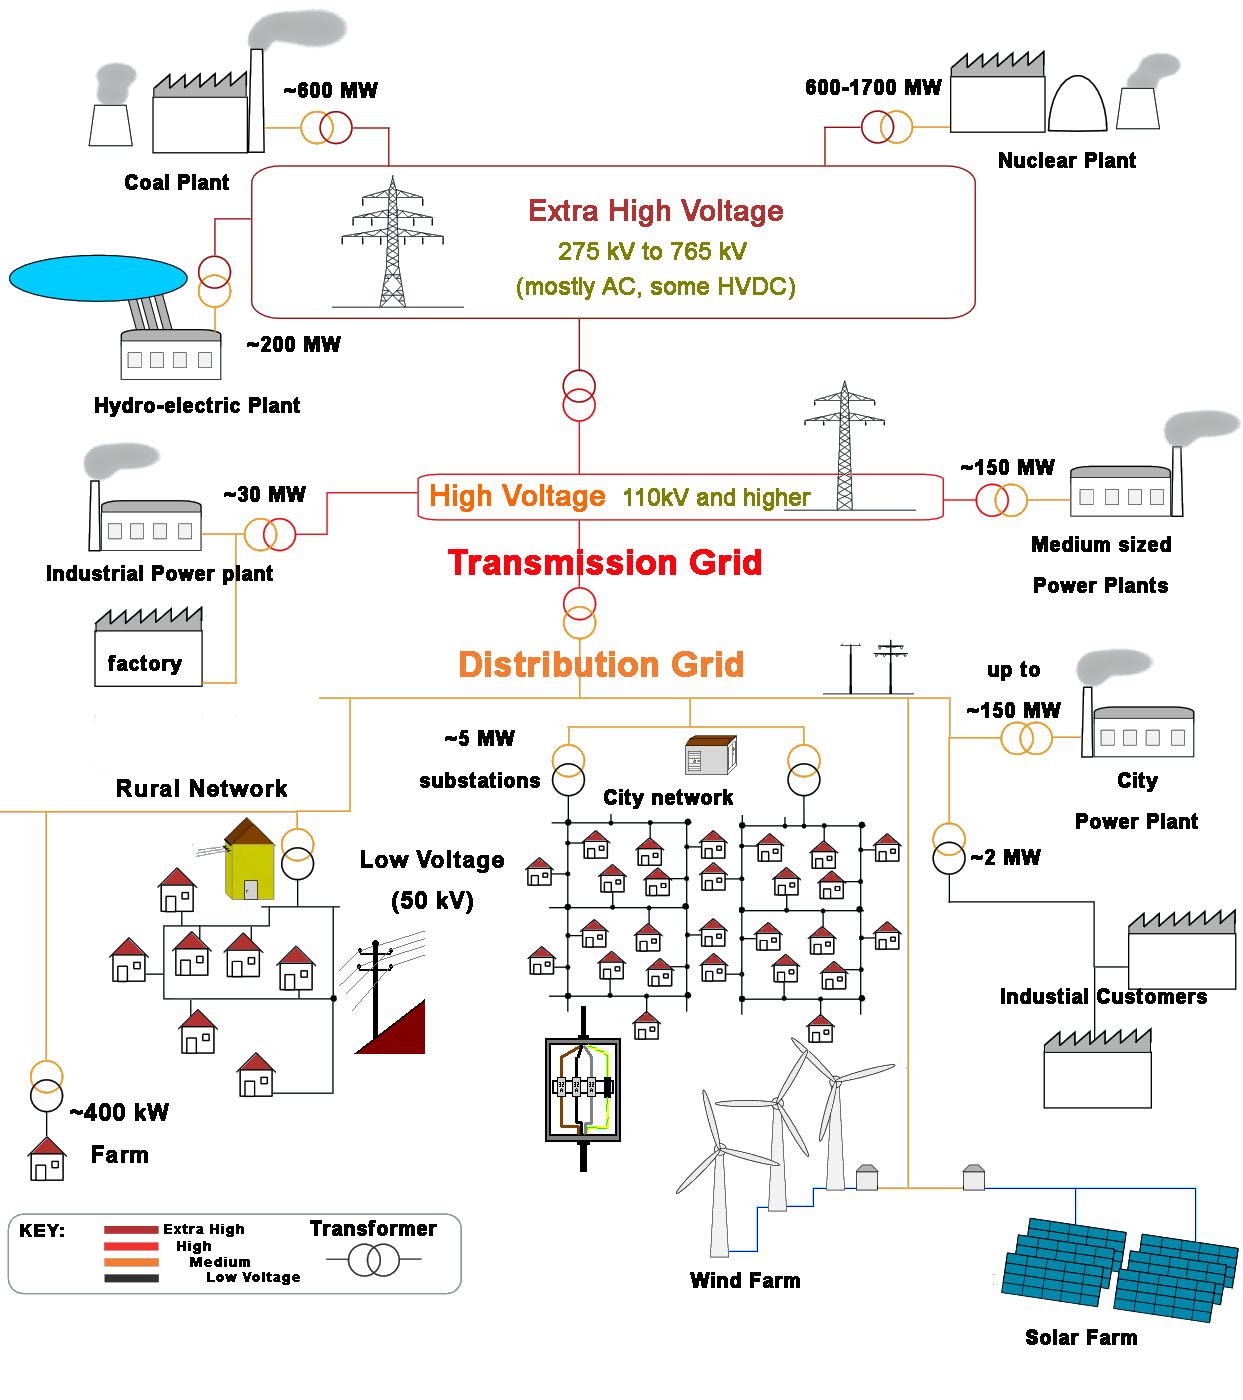
\includegraphics[width=0.8\textwidth]{files/power_system.jpg}
	\caption[Schematic diagram of the power system.]{Schematic diagram of the power system. From Quark64, licensed under a CC-BY-3.0}
	\labfig{ps}
\end{figure}

\begin{kaobox}[frametitle=Task]
Have a look at \reffig{ps}. What three different types of elements of a power system can you identify? How is the system changing now and in future?
\end{kaobox}


\begin{definition}
\labdef{eps}
An electric power system is a network of electrical components that is deployed to supply, transmit, and use electric power for various purposes \sidecite{qazi_chapter_2017}. It consists of three types of elements that
\begin{itemize}
\item generate electricity,
\item transfer electricity (transmission \& distribution), or
\item use electricity.
\end{itemize} 
\end{definition}



\paragraph*{Balancing a power system.}


\begin{kaobox}[frametitle=Task]
One could say our \textit{apple system} is very similar: there are generators, i.e., farms where apples grow, a transfer system, i.e., vans transporting apples, and users, i.e., people eating apples. What are the major differences between the \textit{apple system} and the power system?
\end{kaobox}

A very important characteristic of power systems, especially when considering future renewable and sustainable power systems, is the balance of supply and demand. In contrast to other commodities, e.g., apples, electricity cannot be stored easily. For the power system to be operated in a stable manner, the generation and consumption of electricity in a power system need to be balanced in every moment. That is, the demand of electricity in a certain second, e.g., from a kettle, needs to be matched by power plants generating the same amount of electricity in that same second, e.g., from a wind turbine.


\section{How does a power system model look like?}


% TODO: potentially add more information on structure/equations, input data/data sources/assumptions with regard to power system models

\paragraph*{Building a power system model.}
\begin{kaobox}[frametitle=Task]
A remote mountain cottage in the Scottish Highlands needs a new, sustainable power supply system. The electricity usage is very low but it is needed for light and a few other purposes. The electricity consumption has been measured in the past and is similar every day. The table below gives the power demand for each hour of this typical day.

% TODO: add side note explaining capacity factor

The cottage is not connected to the national electricity grid but there is space to install solar PV panels on the roof, small wind turbines next to the cottage, and a biodiesel generator. The actual generation of the PV panels and wind turbines depends on the weather and the table below gives the capacity factor for solar panels  $CF_S$  and wind turbines $CF_W$ for each of the hours.



\begin{tabular}{ c c c c }

	\toprule
	Hour(s) & Demand (kW) & $CF_W$ (-) & $CF_S$ (-) \\
	\midrule
	00:00 $\rightarrow$ 08:00 & 0 & 0.4 & 0.0\\
	08:00 $\rightarrow$ 09:00 & 0 & 0.3 & 0.1\\
	09:00 $\rightarrow$ 10:00 & 0 & 0.2 & 0.3\\
	10:00 $\rightarrow$ 11:00 & 2 & 0.1 & 0.5\\
	11:00 $\rightarrow$ 12:00 & 4 & 0.0 & 0.7\\
	12:00 $\rightarrow$ 13:00 & 3 & 0.2 & 0.9\\
	13:00 $\rightarrow$ 14:00 & 1 & 0.4 & 0.8\\
	14:00 $\rightarrow$ 15:00 & 0 & 0.5 & 0.7\\
	15:00 $\rightarrow$ 16:00 & 2 & 0.6 & 0.55\\
	16:00 $\rightarrow$ 17:00 & 1 & 0.7 & 0.2\\
	17:00 $\rightarrow$ 18:00 & 3 & 0.6 & 0.1\\
	18:00 $\rightarrow$ 19:00 & 5 & 0.7 & 0.0\\
	19:00 $\rightarrow$ 20:00 & 1 & 0.6 & 0.0\\
	20:00 $\rightarrow$ 24:00 & 0 & 0.3 & 0.0\\
	\bottomrule
\end{tabular}\\


\textbf{Part 1:} Two different engineering consultancy companies develop suggestions for the power supply system of the mountain cottage. Consultancy A suggests to install 2 kW of solar PV, 10 kW of wind turbines, and a 1.5 kW biodiesel generator as backup. Company B suggests to install 4 kW of solar PV, 6 kW of wind turbines, and a 2 kW biodiesel generator. Check if the suggested power supply systems would be able to satisfy the power demand on the mountain cottage! You can use the table below for your calculations.

\begin{tabular}{ c c c c c c c }

	\toprule
	& \multicolumn{3}{c}{Consultancy A}& \multicolumn{3}{c}{Consultancy A}\\
	Hour(s) & $G_W$ & $G_S$ & $G_B$  & $G_W$  & $G_S$  & $G_B$   \\
	& \multicolumn{6}{c}{(kWh)}   \\
	\midrule
	00:00 $\rightarrow$ 08:00 & \line(1,0){14}& \line(1,0){14} & \line(1,0){14} & \line(1,0){14}& \line(1,0){14} & \line(1,0){14}\\
	08:00 $\rightarrow$ 09:00 & \line(1,0){14}& \line(1,0){14} & \line(1,0){14} & \line(1,0){14}& \line(1,0){14} & \line(1,0){14}\\
	09:00 $\rightarrow$ 10:00 & \line(1,0){14}& \line(1,0){14} & \line(1,0){14} & \line(1,0){14}& \line(1,0){14} & \line(1,0){14}\\
	10:00 $\rightarrow$ 11:00 & \line(1,0){14}& \line(1,0){14} & \line(1,0){14} & \line(1,0){14}& \line(1,0){14} & \line(1,0){14}\\
	11:00 $\rightarrow$ 12:00 & \line(1,0){14}& \line(1,0){14} & \line(1,0){14} & \line(1,0){14}& \line(1,0){14} & \line(1,0){14}\\
	12:00 $\rightarrow$ 13:00 & \line(1,0){14}& \line(1,0){14} & \line(1,0){14} & \line(1,0){14}& \line(1,0){14} & \line(1,0){14}\\
	13:00 $\rightarrow$ 14:00 & \line(1,0){14}& \line(1,0){14} & \line(1,0){14} & \line(1,0){14}& \line(1,0){14} & \line(1,0){14}\\
	14:00 $\rightarrow$ 15:00 & \line(1,0){14}& \line(1,0){14} & \line(1,0){14} & \line(1,0){14}& \line(1,0){14} & \line(1,0){14}\\
	15:00 $\rightarrow$ 16:00 & \line(1,0){14}& \line(1,0){14} & \line(1,0){14} & \line(1,0){14}& \line(1,0){14} & \line(1,0){14}\\
	16:00 $\rightarrow$ 17:00 & \line(1,0){14}& \line(1,0){14} & \line(1,0){14} & \line(1,0){14}& \line(1,0){14} & \line(1,0){14}\\
	17:00 $\rightarrow$ 18:00 & \line(1,0){14}& \line(1,0){14} & \line(1,0){14} & \line(1,0){14}& \line(1,0){14} & \line(1,0){14}\\
	18:00 $\rightarrow$ 19:00 & \line(1,0){14}& \line(1,0){14} & \line(1,0){14} & \line(1,0){14}& \line(1,0){14} & \line(1,0){14}\\
	19:00 $\rightarrow$ 20:00 & \line(1,0){14}& \line(1,0){14} & \line(1,0){14} & \line(1,0){14}& \line(1,0){14} & \line(1,0){14}\\
	20:00 $\rightarrow$ 24:00 & \line(1,0){14}& \line(1,0){14} & \line(1,0){14} & \line(1,0){14}& \line(1,0){14} & \line(1,0){14}\\
	\bottomrule
\end{tabular}\\

The table below gives the relevant cost parameters for the three power generation technologies

\begin{tabular}{ c m{2.5cm} m{2.5cm} m{2cm} }
	\toprule
	Technology & Annualized capital cost (\pounds/kW) & Variable cost (incl. fuel) (\pounds /kWh) & Efficiency (-)\\
	\midrule
	PV & 49 & 0 &  1 \\
	Wind & 75 &  0 &  1 \\ 
	Biodiesel & 141 & 0.015 &  0.6 \\
	\bottomrule
\end{tabular}

\textbf{Part 2:} What is the cost-optimal power supply system for the mountain hut? Solve this together with your course leader using a power system model.
\end{kaobox}



\paragraph*{Reflecting on power system models.}~\\


As discussed in \refsec{models}, models are always a simplification of reality built for a particular purpose. Thus, it is always important to make sure the model is fit for the specific purpose it is used for and that one does not draw conclusions from model results that cannot be justified. Moreover, it is also crucial to be aware of and acknowledge the weaknesses of the models and model-based analysis.

\begin{kaobox}[frametitle=Task]
Think about the analysis with regard to the mountain cottage above. Do you think the model is based on realistic assumptions? What are the weaknesses of the analysis?
\end{kaobox}



\section{Homework}
In order to develop useful models, it is important to have a good understanding of the system to be modelled. Perform a short literature research on highly renewable power systems using a scientific search engine (for example, \href{https://scholar.google.com/}{https://scholar.google.com/}. Try to find at least 3 relevant publications, e.g., journal papers or reports, read (at least) the respective abstracts, and write a short summary of around 150-200 words. You can touch on one or more of following points (you do \textbf{not} need to cover all of them):
\begin{itemize}
\item What are the challenges associated with highly renewable power systems?
\item What are potential solutions to address those challenges?
\item What other developments within the power sector play a role?
\end{itemize}

Make sure that you use references to point to your sources. 

% TODO: add side note or otherwise more information on referencing in the handbook
